\documentclass[twocolumn,numberedappendix]{../aastex6}

% these lines seem necessary for pdflatex to get the paper size right
\pdfpagewidth 8.5in
\pdfpageheight 11.0in

% for the red MarginPars
\usepackage{color}

% some extra math symbols
\usepackage{mathtools}

% allows Greek symbols to be bold
\usepackage{bm}

% allows us to force the location of a figure
\usepackage{float}

% allows comment sections
\usepackage{verbatim}

% Override choices in \autoref
\def\sectionautorefname{Section}
\def\subsectionautorefname{Section}
\def\subsubsectionautorefname{Section}

% MarginPars
\setlength{\marginparwidth}{0.75in}
\newcommand{\MarginPar}[1]{\marginpar{\vskip-\baselineskip\raggedright\tiny\sffamily\hrule\smallskip{\color{red}#1}\par\smallskip\hrule}}

\newcommand{\msolar}{\mathrm{M}_\odot}

% Software names
\newcommand{\amrex}{\texttt{AMReX}}
\newcommand{\boxlib}{\texttt{BoxLib}}
\newcommand{\castro}{\texttt{CASTRO}}
\newcommand{\microphysics}{\texttt{Microphysics}}
\newcommand{\wdmerger}{\texttt{wdmerger}}
\newcommand{\python}{\texttt{Python}}
\newcommand{\matplotlib}{\texttt{matplotlib}}
\newcommand{\yt}{\texttt{yt}}
\newcommand{\vode}{\texttt{VODE}}
\newcommand{\isoseven}{\texttt{iso7}}
\newcommand{\aproxthirteen}{\texttt{aprox13}}
\newcommand{\aproxnineteen}{\texttt{aprox19}}
\newcommand{\aproxtwentyone}{\texttt{aprox21}}

\begin{document}

%==========================================================================
% Title
%==========================================================================
\title{White Dwarf Mergers on Adaptive Meshes\\ II. Nuclear Reactions}

\shorttitle{WD Mergers. II. Nuclear Reactions}
\shortauthors{Katz et al. (2017)}

\author{Max P. Katz\altaffilmark{1}}
\author{Michael Zingale\altaffilmark{1}}
\author{Alan C. Calder\altaffilmark{1,2}}
\author{F. Douglas Swesty\altaffilmark{1}}
\author{Ann S. Almgren\altaffilmark{3}}
\author{Weiqun Zhang\altaffilmark{3}}
\author{Frank X. Timmes\altaffilmark{4,5}}

\altaffiltext{1}
{
  Department of Physics and Astronomy,
  Stony Brook University, Stony Brook, NY, 11794-3800, USA
}

\altaffiltext{2}
{
  Institute for Advanced Computational Sciences,
  Stony Brook University, Stony Brook, NY, 11794-5250, USA
}

\altaffiltext{3}
{
  Center for Computational Sciences and Engineering,
  Lawrence Berkeley National Laboratory, Berkeley, CA 94720
}

\altaffiltext{4}
{
  The Joint Institute for Nuclear Astrophysics, USA
}

\altaffiltext{5}
{
  School of Earth and Space Exploration, Arizona State University, Tempe, AZ, USA
}



%==========================================================================
% Abstract
%==========================================================================
\begin{abstract}
Simulations of white dwarf mergers that include thermonuclear reactions must
confront the question of how nuclear detonations form and whether observed
detonations in a numerical simulation are realistic. We address this question
by performing simulations of collisions of white dwarfs, a subset of white
dwarf mergers that occur when the stars approach each other nearly head-on.
These have the potential for explosive nucleosynthesis, leading to a thermonuclear
detonation that disrupts both stars, possibly causing a Type Ia supernova.
While this story is intuitively plasible, demonstrating this in a reacting
hydrodynamics simulation is challenging due to the rapid evolution of the
nuclear burning, posing numerical challenges related to both spatial and
temporal resolution. In this study we explore a number of the algorithmic choices
that affect the outcome of reacting hydrodynamics simulations, and address
the question of what is required to ensure that these simulations are properly
converged. We find that achieving a converged white dwarf collision simulation
in the code \castro\ is very difficult. The typical timesteps taken by hydrodynamics
codes are too large, and the achievable spatial resolution is too low, while increasing
either to the point required to actually obtain a converged simulation is
prohibitive. We have identified a criterion for adaptive mesh refinement
that covers the most important regions in the simulation and allows us to
achieve very high resolution in the burning region. However, even in our
highest resolution simulations, we do not find a converged result, and
detonations seem to occur stochastically. Our results point to a path forward
for astrophysical simulations with thermonuclear detonations, but for now
they encourage severe caution in interpreting observed detonations in previous
and current simulations.
\end{abstract}
\keywords{supernovae: general - white dwarfs}

%==========================================================================
% Introduction
%==========================================================================
\section{Introduction}
\label{sec:introduction}

Binary white dwarf (WD) systems are a promising progenitor candidate for Type
Ia supernovae (SNe Ia) for observational reasons, but from the simulation
perspective there is still significant uncertainty regarding how nuclear
detonations form in an exploding white dwarf. There is uncertainty in the
model, regarding whether detonations form on the surface of a star as
accreting material heats up when it strikes the surface, or at or near the
center of the star as the accreted material compresses the WD. There is also
uncertainty in the numerics: given one of these models, can we self-consistently
demonstrate that a detonation occurs? This question has haunted both single
WD and double WD progenitor models, because the length and time scale at which
a detonation forms is orders of magnitude smaller than the resolution that
typical hydrodynamic simulations can achieve. Furthemore, the approximate equations
we use at the resolution that we can achieve are still notoriously
difficult to solve accurately. The mere presence of a detonation
(or lack thereof) in a simulation is therefore only weak evidence regarding
whether a detonation would truly occur.

In this study we examine the challenges associated with simulating nuclear detonations.
This paper follows from our first WD merger methodology paper, \citet{wdmergerI}
(hereafter, Paper I), where we deferred discussion of our nuclear reaction methodology.
After presenting the burning methodology, we apply it to the problem of collisions of white dwarfs.
WD collisions can occur in isolated binaries or in hierarchical triple systems, where the WD binary
system in a tight inner orbit is gravitationally coupled to a third, outer star \citep{thompson:2011,hamers:2013}.
Whether the rate of these collisions may be high enough to significantly contribute to
the observed SN Ia rate is debated: \cite{katzdong:2012} suggest that this is plausible,
but \cite{hamers:2013} and \cite{papish:2015} suggest that the rate is relatively low.
Regardless, they are a useful vehicle for understanding the problem of nuclear burning.
Head-on WD collisions rapidly convert a significant amount of kinetic energy into thermal
energy in a small region and thus set up conditions ripe for a thermonuclear detonation;
being able to correctly simulate these is in some sense a prerequisite to correct simulation
of the more complicated general case of white dwarf mergers, where we do not initially know
under what conditions the seed of a thermonuclear detonation is born.

There have been a number of previous studies which provide useful insight into setting up
the problem and the burning methodology \citep{rosswog:2009,raskin:2010,loren-aguilar:2010,
hawley:2012,garcia-senz:2013,kushnir:2013,papish:2015,holcomb:2015}. These studies
found that detonations occur and convert a large amount of carbon/oxygen material into
iron-group elements. These papers varied significantly in the hydrodynamic methods used
(Lagrangian versus Eulerian methods), the methodology used for coupling nuclear
reactions to the hydrodynamics (including variation in the number of isotopes in
the nuclear network and in the evolution of the temperature), and the temporal and
spatial resolution. Consequently the detonations they formed varied in location and nature,
and the resultant estimates of production of nickel-group elements varied significantly,
leaving much uncertainty about how such an event would appear observationally and whether
it bears any resemblance to a SN Ia. See Table 4 of \cite{garcia-senz:2013} for a summary
of the outcome of many of these studies. In this paper we make the case that
while we can identify the main problems prevent accurate simulation of the collision
event, there is no clear path to overcoming them using the computational resources
typically available for contemporary hydrodynamics simulations.



%==========================================================================
% Problem Setup
%==========================================================================
\section{White Dwarf Collisions}
\label{sec:collisions}

We start with a description of the problem setup and results of a typical collision
at low resolution. These results set the stage for our numerical methodology. This enables
a concrete discussion about the methodology using the language of how it affects the
collision outcome. In this setting, a concrete discussion is more fruitful than an abstract one.



\subsection{Problem Setup}
\label{sec:problemsetup}

We implement the white dwarf collision problem in \castro\ in the \wdmerger\ problem
directory. We prepare the domain in the way most previous papers have done so:
the white dwarf centers of mass are initially separated by a distance of four times
the (secondary) white dwarf radius. Note that the radius of the white dwarf, and
consequently the initial distance, depends on the equation of state used, and this
can vary somewhat depending on the relevant physics used, such as Coulomb corrections
in the Helmholtz equation of state. However, the results do not really depend on the
exact initial distance as long as there is enough time for the WDs to distort in
response to tidal forces as they approach. Their initial velocity is that of
two point-masses in free-fall towards each other coming in from infinity, such that
the contact point is at the origin, and they approach each other along a coordinate axis.
In this paper we focus only on head-on collisions of two 0.64 $\msolar$ white dwarfs
composed of equal parts carbon and oxygen by mass, at an initially uniform temperature
of $T = 10^7$ K. This choice is for comparison to earlier studies; the code does have
the ability to vary the impact parameter of the collision and the mass and composition
of the WDs.

We have added to the \wdmerger\ problem setup the ability to take advantage of 
the 2D cylindrical ($R-z$) coordinate system evolution in \castro, and we use it
in this study, because the axisymmetry inherent to the cylindrical coordinate system
lends itself well to the head-on collision problem. In this coordinate system, we
align the WDs along the $z$-axis (which is analogous to the $x$-axis in Cartesian
evolution), with the center of the WDs at $R = 0$. The un-simulated $\phi$ dimension
then would extend the WDs through a $2\pi$ revolution. The domain has width $4 \times 10^{9}$
cm along the $z$ axis, and is half as wide along the $R$ axis. The resolution is equal
in both dimensions, so that there are twice as many zones in the $z$ dimension in
a uniform grid.

We terminate the simulation at $t = 9$ seconds, as we have found that for this
particular setup, all of the significant burning has completed by this time\footnote{In
some simulations we were mainly interested in seeing when the detonation happened, and
we terminated the simulation at that point. We show nucleosynthesis results only for
those simulations that had completed nuclear burning.}. At
this point, the total energy on the domain has become positive, typically about
$10^{51}$ ergs, and has stopped increasing. This means that the system has become
unbound due to nuclear energy release, and that no further meaningful nuclear energy
generation is occurring. In our discussions below, it helps to have some other
anchoring points in time when significant events occur. We arbitrarily define the
collision time, $t_{\rm c}$, as the time when the density at the center of the grid
first reaches $10^2\ \text{g\,/\,cm}^3$. This is reached only when the WDs meet at the
center of the domain. We define the detonation time, $t_{\rm d}$, as the time when the
temperature first reaches $4.5 \times 10^9\ \text{K}$. This is also an arbitrary
threshold, but we have found empirically that this temperature is only reached in
the collision when a detonation is formed.

The region outside the WDs is filled with a low-density ambient
material with $\rho = 10^{-4}\ \text{g\,/\,cm}^{3}$ whose composition and temperature is the
same as that of the WDs. Reactions in this region are unimportant, so for
computational efficiency, we disable all nuclear burning for zones that have
$\rho < 10^6\ \text{g\,/\,cm}^{3}$ and $T < 10^8\ \text{K}$. We have confirmed that
the results do not depend on this choice. A sponge is applied to all gas of density
lower than $1\ \text{g\,/\,cm}^{3}$. The sponge damps out the velocity in these zones
(see Paper I) to prevent spurious numerical error in low-density gas from dragging
down the global timestep. The density floor for the simulation is set
at $10^{-5}\ \text{g\,/\,cm}^{3}$ and the temperature floor is $10^7$ K.

Our primary metric for this test is the amount of $^{56}$Ni generated in the collision,
as this is the parameter most directly related to the observable quantities of interest
for Type Ia supernovae. We collect information at the end of every timestep about the
total amount of nickel on the grid (in solar masses), and we use the maximum value of
this nickel mass. Plotfiles of relevant quantities are created every 0.01 seconds.
The timesteps are limited to ensure that every multiple of this plotfile interval is
reached exactly, which means an effective maximum timestep of 0.01 seconds.



\subsection{Baseline Results}
\label{sec:baseline_results}

Now let us examine the results for a collision of two 0.64 $\msolar$ WDs. We use
128 zones in the radial dimension, corresponding to a spatial resolution of 312.5 km.
Timesteps are limited only by the hydrodynamic stability constraint (and the plotfile
interval constraint). Resolutions in the range of a few hundred km have been a common
choice in earlier papers on white dwarf mergers and collisions. No adaptive mesh
refinement is used. For this configuration, the collision time is approximately $t_{\rm c} = 4.6\ \text{s}$,
and the detonation time is $t_{\rm d} = 7.43\ \text{s}$. The peak density at the detonation time
is $2.3 \times 10^7\ \text{g\,/\,cm}^3$. The detonation occurs at the center of the domain
where the two WDs initially meet.



%==========================================================================
% Numerical Implementation
%==========================================================================
\section{Numerical Methods}
\label{sec:numericalmethods}

The hydrodynamical equations solved in this paper were presented in \citet{wdmergerI}
(hereafter, Paper I) for the reacting hydrodynamics code \castro\ \citep{castro}.
Only minor revisions to the core hydrodynamic algorithm have since occurred.
In this paper we focus our discussion on our implementation of the nuclear
reaction network and integrator. There are three main areas of concern: first,
specifying what nuclides are in the network and what reaction rates link the
various nuclides; second, once the system of ODEs governing the evolution of
the nuclear species has been written down, how to couple them to ODEs governing
the evolution of the thermodynamics, in particular the temperature; third,
coupling the nuclear reaction updates to the evolution of the hydrodynamical
system. We will deal with each of these in turn in the following subsections.

\subsection{Nuclear Network}
\label{sec:network}

White dwarfs are primarily composed of the $\alpha$-chain particles ${}^4$He,
${}^{12}$C, ${}^{16}$O, ${}^{20}$Ne, and ${}^{24}$Mg. Therefore the core of
any network appropriate for modeling nuclear burning in white dwarfs will be
these alpha chain nuclides, with the idea being that links up the $\alpha$-chain
will eventually get us to ${}^{56}$Ni, the nuclide responsible for the
energy output of Type Ia supernovae. In this paper we use the \aproxthirteen\
network\ \citep{timmes:1999,timmes:2000}. This includes all thirteen $\alpha$-chain
particles between ${}^4$He and ${}^{56}$Ni. This network was used by \citet{hawley:2012}
and \citet{raskin:2010}. \citet{loren-aguilar:2010} and \citet{garcia-senz:2013} used a
very similar network that additionally included ${}^{60}$Zn. This network has been
ported into a form that is consistent with the \amrex\ codes, in the freely available
\microphysics\ code repository
\footnote{\microphysics\ can be obtained at \url{https://github.com/starkiller-astro/Microphysics}.},
a collection of microphysical routines that are designed to be used in our
hydrodynamics codes. In our \microphysics\ repository we have also ported \aproxnineteen\
\citep{timmes:1999}, which was used in a few previous collision papers, and \aproxtwentyone.
The isotopes added by these networks relative to \aproxthirteen\ are not particularly relevant
to the problem of head-on white dwarf collisions, so we do not discuss results with these networks
here (though we have verified for this problem that these larger networks do not significantly change
the answer). We also make available \isoseven\ \citep{timmes:2000}, which skips the nuclides between
silicon and nickel, and was used by \citet{rosswog:2009}. \isoseven\ gives significantly different
quantitative results than \aproxthirteen\ for this problem, due to the inapplicable assumption of
an equilibrium abundance of the unused isotopes, but the results are still qualitatively similar.

\subsection{Nuclear Burning}
\label{sec:burner}

Given a set of nuclides and the reaction links between them, we now consider
how a burning step is performed in our software. The goal is to integrate the
vector ${\bm{Y}} = (Y_1, Y_2, \ldots, Y_n, e, T)$, where $Y_{n} = X_{n} / A_{n}$
is the molar fraction of species $n$, with $X_n$ the mass fraction and $A_n$ the
mass number of that species, $e$ is the energy released during the burn, and
$T$ is the temperature. The equation describing its evolution is given by
\begin{equation}
  \frac{d\bm{Y}}{dt} = f(\mathbf{Y}),
\end{equation}
where the components of the right-hand-side for the species come from the particular
nuclear burning network we are using. The energy $e$ of the zone
will change when the nuclear abundances evolve, according to
\begin{equation}
  \frac{\partial e}{\partial t} = N_A \sum_{n} \frac{\partial Y_{n}}{\partial t} m_{n} c^2,
\end{equation}
where $c$ is the speed of light and $m_n$ is the mass of each nuclide.

We define several burning modes that determine how $T$ and $e$ are evolved
during a nuclear burn. In a hydrostatic burn, which we call burning mode 0,
we keep $\rho$ and $T$ fixed throughout, and use 
the energy released at the end to compute a final temperature that is
thermodynamically consistent with the new internal energy. By contrast,
in a self-heating burn (mode 1), we allow the temperature to evolve in response
to the burning (see\footnote{In the cited paper, a term based on the
thermodynamic chemical potential was included; we now believe
that it is incorrect to include such a term in the burn, since it
automatically sums to zero analytically.} \citet{maestro3}):
\begin{equation}
  \frac{dT}{dt} = \frac{1}{c_V}\frac{\partial e}{\partial t}
\end{equation}
(Although $T$ evolves during the burn so that the integration is physically
accurate, as in the hydrostatic method we discard the final value
for $T$ at the end of the burn and recompute a temperature for the zone that is
consistent with its new internal energy.) Here $c_V$ is the specific heat at
constant volume, which is provided by the equation of state.  During this burn,
we can keep $c_V$ constant using its initial value, or at each step we
can choose to re-evaluate the equation of state using the latest value of $(\rho, T)$.
The latter is more expensive but also more accurate, and we use it in this paper.
In practice we find that the cost is small in comparison to the more expensive
parts of the calculation, and it can significantly speed up convergence near NSE.
A third option (mode 2) presented by \citet{raskin:2010} is a so-called ``hybrid'' mode.
In this mode, by default we do a hydrostatic burn. If that burn fails, or if the net
energy change is negative, we do the burn again in self-heating mode. A final option (mode 3)
is a burn that limits the changes due to a burn to avoid numerically unstable burning.
This mode is discussed in \autoref{sec:unstable_burning} and we will call it a
``suppressed'' burn for the remainder of this work. All four options
are implemented in our burner software.

The simulations shown in this work all use the self-heating mode. The hydrostatic
and hybrid burns are only a slight variation on the self-heating burn in practice
for this problem.
The reason that the hydrostatic burn cannot substantially change the outcome is
that even though the temperature is fixed during the burn, it is \textit{not}
constant in the rest of the hydrodynamics step. And in the hydrodynamics step,
the \castro\ algorithm performs multiple EOS calls to ensure that the temperature
is synchronized with the internal energy at various points in the update. So in
practice there is a temperature change due to the burn for our problem. This seems
inevitable for any hydro code unless the hydrodynamics update includes an explicit
equation for $T$ that is independent of what is happening for the internal energy.
The hydrostatic burn does slightly limit the energy release during any given burn,
but summed up over the whole simulation this is not enough to qualitatively affect
the outcome. The hybrid burn does not affect the simulation outcome at all relative
to the hydrostatic burn. The difference between them only applies for zones that have
a net negative energy release from the hydrostatic burn, which occurs only after
we have burned to NSE. The hybrid burn was mainly implemented by \citet{raskin:2010}
for making it easier to numerically complete a burn, rather than because of the
effects it has on the outcome of the simulation. The suppressed burn has separate
issues which we defer to \autoref{sec:unstable_burning}

In our \microphysics\ repository we provide several software options for
solving a set of coupled stiff ODEs. For this work our primary integrator
is the classic \vode\ integrator \citep{vode}, of which we have a version
compatible with our software interfaces in the \microphysics\ repository.
We also employ an implementation of the well known variable-order Richardson
extrapolation method presented by \citet{stoer:1980}, that is similar to the
integrator which ships with the original versions of the networks mentioned
above. Our experience shows that relying on a single ODE integrator for the
variety of stiff ODEs that are present in a collision is insufficient, as we
sometimes run into integration failures. A combination of the two integrators
is usually sufficient, however: we first try \vode, and if that fails, we then
try the Stoer and Bulirsch method. Since it is possible for neither method to
succeed, we have one more backup scheme. Our specified (relative and absolute)
error tolerances are uniformly $10^{-6}$ for the energy, temperature, and nuclear
abundance ODEs. We can loosen these tolerances in an attempt to give the integrator
an easier time. If both \vode\ and the Stoer and Bulirsch algorithm fail, then we
loosen the tolerances by a multiplicative factor of 25\%, and then repeat the attempts
with \vode\ and Stoer and Bulirsch. We keep doing this until either we have loosened
the tolerances enough for one of the two methods to succeed, or until we have loosened
the tolerances by two orders of magnitude, at which point we finally give up. We have
found that this scheme is resilient enough to handle all of the simulations shown below.
We have also verified that our results do not depend strongly on the tolerances when they
are tighter than $10^{-4}$. For the typical collision problem we discuss below, the
nucleosynthetic yield for nickel varies by less than 5\% between a tolerance of $10^{-4}$
and a tolerance of $10^{-12}$.

\subsection{Coupling to the Hydrodynamics}
\label{sec:hydrocoupling}

In \castro, the reactions are coupled to the hydrodynamics using Strang splitting.
In a given timestep advance $\Delta t$, we first evolve the reactions alone through
a time interval $\Delta t / 2$. Then, we evolve the hydrodynamics for $\Delta t$,
and we evolve the reactions again for a further $\Delta t / 2$. The principal
drawback of this approach is that the reactions and the hydrodynamics can become
decoupled from each other. A common solution to this problem presented in
the literature has been to limit the size of the timestep and thereby limit the
extent of this decoupling \citep{raskin:2010,hawley:2012}, which we adopt here 
and have implemented in \castro. Defining the nuclear energy injection timescale 
$\tau_e$, and the species evolution timescale $\tau_{X_k}$,
\begin{align}
  \tau_e &\equiv \frac{e}{|\dot{e}|} \\
  \tau_{X_k} &\equiv \frac{X_k}{|\dot{X_k}|},
\end{align}
where $\dot{e}$ is an estimate of the time rate of change of the internal energy
from nuclear burning, and $\dot{X_k}$ is an estimate of the time rate of change 
of the mass fraction of the species with index $k$, we define burning-limited 
timesteps $\Delta t_{be}$ and $\Delta t_{bX_k}$:
\begin{align}
  \Delta t_{be} &= f_{be}\, \tau_e \label{eq:timestep_e}\\
  \Delta t_{bX_k} &= f_{bX}\, \tau_{X_k}. \label{eq:timestep_X}
\end{align}
Given an estimate for $\dot{e}$, the factor $f_{be}$ determines by what 
fraction we would like to allow the internal energy to change
in the current timestep, under the assumption that $\dot{e}$ does not change from
timestep to timestep. Similarly, given an estimate for $\dot{X_k}$, the factor $f_{bX}$ 
determines the maximum change in the mass fraction of any species. To prevent species
whose abundances are small in absolute terms from controlling the timestep, we apply
the limiter based on $f_{bX}$ only to species with abundances in a given zone greater
than $10^{-3}$ (this abundance threshold can be changed by the user of the code). By making 
$f_{be}$ and $f_{bX}$ smaller, we can control the magnitude of the decoupling 
between the reactions and the hydro. A typical choice for $f_{be}$ in the
literature is in the range of 0.1 to 0.3, while to our knowledge a limiter based on
$f_{bX}$ has not been used by others performing these types of calculations. The sensitivity
of results to the value of these timestep limiters will be discussed in 
\autoref{sec:temporalresolution}. The factors $f_{be}$ and $f_{bX}$ can be set at runtime in \castro.

At the start of each advance, we limit the size of the timestep to be the smaller
of the minimum hydro timestep (limited by the CFL condition), and the minimum of all the
burning timesteps across all zones. To do this, we need a method for determining 
$\dot{e}$ and $\dot{X_k}$. We choose to do this with a direct evaluation of the
right-hand-side of the burning network, given the current state at the time when
the timestep is evaluated. Other work in the literature has typically evaluated
this as a finite difference using the change over the last timestep. Our method
is more accurate in principle, but in practice for this problem we find no
meaningful difference between the limiting we propose and other methods of
estimating the time derivatives.

To be precise, we note that the timestep
will only actually satisfy the energy criterion
$\Delta t \leq f_e \tau_e$ and species criterion
$\Delta t \leq f_{X_k} \tau_{X_k}$ when the estimates for
$\dot{e}$ and $\dot{X_k}$ we generate are at least as large
as the actual rate of change of energy and mass fractions
over the timestep. However, this can assumption will sometimes fail
during periods of runaway burning when the rate of change
of these quantities is highly nonlinear. We may not want
to neglect the errors caused by this approximation
because they may build up over an extended period of nonlinear
evolution and perhaps substantially change the final results.
To this end, we have implemented a timestep retry option in
\castro, which re-computes an advance if it violated the
stability criteria as judged from the end of the timestep,
using subcycled timesteps which individually satisfy the
stability criterion to the tolerance we have asked for.
We have found that the benefits for this problem are, however, small.

%TODO: add a ``Nonaka plot''

To understand the consequences of the timestep limiting, and more broadly to 
understand the limitations of Strang splitting, we consider the 
basic outline of a single-level advance in an advection-reaction system:
\begin{enumerate}
  \item Evaluate timestep $\Delta t$ for the current advance
  \item Advance the nuclear burning network by $\Delta t / 2$
  \item Advance the hydrodynamics by $\Delta t$
  \item Advance the nuclear burning network by $\Delta t / 2$
  \item Return to Step 1
\end{enumerate}
Now, consider that during a head-on collision, initial nuclear burning 
will occur at the contact point between the two stars. Because of 
the staggered updates from splitting, the evolution effectively progresses 
as a cycle between burning for $\Delta t$ and getting fresh material 
advected into the contact point by the hydro update for $\Delta t$. 
When the collision begins, $\Delta t$ is controlled by the hydrodynamic 
stability criterion, and may be large enough that it is possible for 
the burning advance in Step 4 to completely burn the freshly advected 
material all the way to NSE. Consequently the evolution is no longer 
a good approximation to smooth burning of the in-falling material but
rather separate discrete burning and hydro steps, and the nature of 
the burning evolution will be quite different. As the timestep becomes
smaller, the evolution becomes smoother and the splitting error decreases.

\begin{figure}[ht]
  \centering
  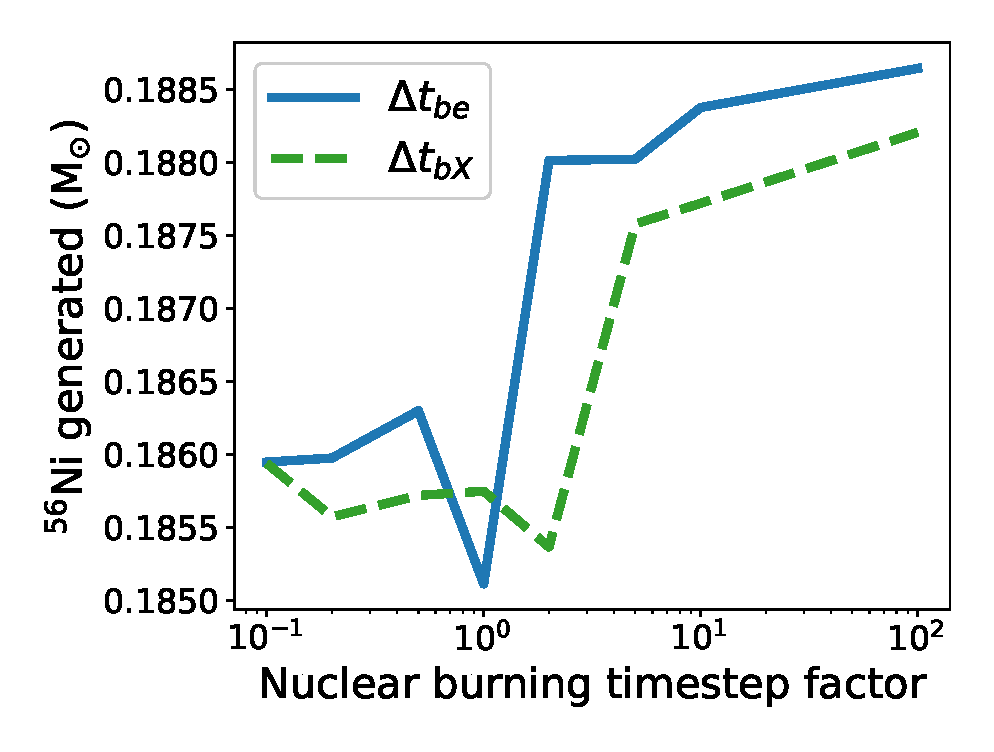
\includegraphics[scale=0.425]{{{plots/dtnuc_max_Ni56_m_P_0.64_m_S_0.64}}}
  \caption{Nickel production as a function of the timestep factors $f_{be}$
           (solid blue, limiting the timestep on changes in internal energy) and
           $f_{bX}$ (dashed green, limiting the timestep on changes in species).
           For a given $f_{be}$, $f_{bX}$ with the same value typically limits
           the timestep by at least an order of magnitude more.
           \label{fig:timestep_factor}}
\end{figure}
\autoref{fig:timestep_factor} demonstrates the effect of both parameters on the nickel
production for the baseline collision case. These limiters are somewhat redundant in
the sense that a given $f_{bX}$ roughly corresponds to another (higher) $f_{be}$, as
is evident by the fact that on the plot the curves look qualitatively similar in
shape but with a horizontal offset. As either $f$ becomes small, the restriction on
the timestep becomes more severe: for $f_{bX} = 0.1$, the full simulation requires
nearly 30,000 timesteps, compared to just over 1,000 for the baseline case.
Such a simulation would be quite expensive for a high resolution 3D calculation.
It is clear, though, that even though the simulation is not converged when the
timestep is not limited due to burning, the effect is small in absolute terms.
So we agree that the use of values in this range by \cite{raskin:2010},
\cite{hawley:2012}, and \cite{kushnir:2013} is appropriate. However, for reasons of
computational expense we do not use the timestep limiter in the high resolution
simulations that follow. The error due to this choice should be small, because
the effect is not that large to begin with, and because the higher resolution
decreases the timestep anyway due to the hydrodynamic stability constraint.

Other approaches to the coupling 
between reactions and hydrodynamics have been proposed in the 
broader literature, especially iterative methods such as 
deferred corrections that allow each of these operators to 
feel the lagged effects of the other operators. For example,
in the context of low Mach number flows, \cite{nonaka:2012} have
used the method of spectral deferred corrections \citep{SDC} to
couple their advection-diffusion-reaction equation set. In our
context this would involve treating the full evolution equation
for each of the state variables as an ODE with a directly coupled
burning source term integrated at high order; the advective
flux is evaluated at the standard second order accuracy
and is included as an ODE source term.
We are presently investigating such a method,
and it may form the basis of further work on this subject.

\subsection{Numerically Unstable Burning}
\label{sec:unstable_burning}

\citet{kushnir:2013} point out that an inappropriate timestep is 
not the only way for the numerical discretization to cause 
severe errors in the burning. Another possible failure mode is when
the energy injection timescale
$\tau_e$ is shorter than the sound-crossing time $\tau_s$ in a zone.
When the sound-crossing time is too long, energy is built up in
a zone faster than it can be advected away by pressure waves.
This is of course a problem inherent only to numerically discretized
systems as the underlying fluid equations are continuous.
This can lead to a numerically seeded detonation caused by the
temperature building up too quickly in the zone; the detonation
may be spurious in this case. If the following condition holds,
we can be confident that a numerically seeded detonation has not occurred:
\begin{equation}
  \tau_s \leq f_{s}\, \tau_e \label{eq:burning_limiter_2}
\end{equation}
The sound crossing time, $\tau_s$, is given by $\Delta x / c_s$, 
where $c_s$ is the sound speed and $\Delta x$ is the (minimum) 
zone width. The parameter $f_{s}$ then determines the minimum
ratio of the nuclear energy generation timescale to the 
sound-crossing time. \citet{kushnir:2013} choose $f_{s} = 0.1$ 
for their simulations. \citet{kushnir:2013} implemented this
criterion by artificially limiting the magnitude of the energy
release after a burn.

To understand this choice, consider the outcome of our baseline case.
When the two WDs collide, there is a prompt detonation
at the contact point at the center of the domain. This detonation occurs
when the density is relatively low because the WDs have not had much
time to collide, and so the nucleosynthetic yield of nickel is low. If
this is the case, the colliding WDs are not a good candidate for
normal SNe Ia. However, if this detonation is delayed, material builds
up at a stalled shock in the center, and the eventual detonation occurs
on the outer edge of the stalled shock. There will then be much more
high density material to process into nickel, and the resulting
explosion creates an amount of nickel potentially sufficient to explain
normal SNe Ia. The discussion thus centers on whether the prompt detonation
is physical. \citeauthor{kushnir:2013} argues that it is not, on the basis
that $\tau_s > \tau_e$ when this detonation occurs. We find the same thing:
for the baseline case, the sound-crossing time is about five times longer
than the energy injection time. This means that a detonation is guaranteed
to occur for numerical reasons. \citeauthor{kushnir:2013} thus argue that
the suppressed burn is justifiable, as it suppresses this prompt detonation.

This argument is flawed because a physical detonation may \textit{also}
occur this way. For example, consider a region of WD material at uniformly
high temperature, say $5 \times 10^9\ \text{K}$, with an arbitrarily large size,
say a cube with side length 100 km. This region will very likely detonate,
even if it is surrounded by much cooler material. By the time the material on
the edges can advect heat away, the material in the center will have long since
started burning carbon, as the sound crossing time scale is sufficiently large
compared to the energy injection time scale. This is true regardless of whether
the size of this cube corresponds to the spatial resolution in a simulation.
Suppression of the burn in this case is unphysical: if we have a zone matching
these characteristics, the zone should detonate.

It is true that when our resolution is low enough, there is a floor on the size
of a hotspot, possibly making such a detonation more likely. However, this is an
unavoidable consequence of the low resolution: it is the correct result of the
simulation that was performed. If the results do not match what occurs at higher
resolution, then the simulation is not converged and the results are not reliable.
However, it may also be the case that a higher resolution simulation will yield
similar results, for example because even at the higher resolution, the physical
size of the hotspot stays the same. Additionally, one might think that simply
adding adaptive mesh refinement in the burning region could help, because then
$\Delta x$ decreases, so the ratio of $\tau_s$ to $\tau_e$ should decrease.
We developed an AMR criterion to do just this: we tag on regions suggested by
the burning stability criterion, \autoref{eq:burning_limiter_2}. But
if a low resolution simulation develops a very large hotspot that violates the
stability criterion, adding refinement inside this region will likely not help,
because the energy trapped in the center of the region may not be able to escape
before ignition occurs. So for low resolution simulations, even adding a significant
amount of refinement (say, refining by a factor of 64 or 128) did not change the
propagation of a detonation.

For the above reasons, an appeal to the numerical instability criterion alone is
insufficient to understand whether a given ignition is real. We find that \textit{all}
of the detonations we have seen at low and moderate resolution inevitably violate
the stability criterion. This is true even if the prompt detonation is suppressed:
the delayed detonation also is numerically unstable. For comparison purposes, we
developed an option for our burner to use a ``suppressed'' burning mode. In a
suppressed burn, we limit the changes to the state so that \autoref{eq:burning_limiter_2}
is always satisfied\footnote{To achieve this we directly multiply the
right-hand-side vector in the integration by a factor $F$
for all variables, where $F$ is the multiplicative factor needed to
be applied to $\dot{e}$ such that the equality in \autoref{eq:burning_limiter_2}
holds. (If the inequality is already satisfied, then the integration
vector is not modified.) We fix $\tau_s$ to be the value of the sound
crossing time at the beginning of the burn (that is, we do not
update it as the sound speed changes) and we fix the energy $e$
that goes into the estimate for $\tau_e$ to be the value of the
internal energy of the zone at the beginning of the burn.}. When we
evolve the baseline case with this suppressed burner, the prompt detonation
is indeed suppressed. A later detonation does occur, but this delayed
detonation also triggers the suppression. The result is that the detonation
does not get to very high temperatures, and the result is again a ``failed''
supernova that does not generate nearly enough nickel. Thus we do not
reproduce the claim of \citeauthor{kushnir:2013} that the suppressed
burning mode suppresses only the prompt detonation, but allows the
delayed detonation to occur. We could find some way to turn off the
suppression and allow the delayed detonation, but without some independent
confirmation that the delayed detonation is physical (while the prompt
detonation is not) this would be begging the question.

The upshot of this discussion is that the only way to resolve the
question is with higher resolution simulations. The semi-analytic
criterion provided by \cite{garg:2017}, and the numerical calculations
of \cite{seitenzahl:2009}, give critical radii for spontaneous detonation.
For the densities we are interested in ($\sim 10^7\ \text{g\,/\,cm}^3$),
assuming equal C/O material, the critical radii are in the range 1-10 km.
So, as pointed out by \citeauthor{kushnir:2013}, this numerical
stability issue is mainly a concern for simulations with
resolution of O(10 km) or worse. Detonations observed at higher
resolution are physically plausible because the critical temperature
gradient will be resolved. The high resolution needs to be achieved
with some combination of high resolution of the collision process
itself, and perhaps AMR based on the stability criterion as described
above, where we tag for refinement all zones above some $f_{s}$, the
ratio of the sound crossing time to the energy injection time. It
cannot be solely based on the burning stability criterion for the reason
described above, that a detonation may be spuriously locked in by
the low resolution regardless of how much resolution we add to it.



%==========================================================================
% Resolution Dependence
%==========================================================================
\section{Spatial Resolution}
\label{sec:spatialresolution}

Now we turn to an examination of the effect of spatial resolution on the detonation.
The first question we want to answer is: at reasonable uniform spatial resolution, is
the simulation converged when a detonation occurs? If the answer is no, then the
follow-up question is: can adaptive mesh refinement help achieve a converged simulation?

To answer these questions we performed a series of simulations at varying base
resolutions, augmented with additional runs with AMR. In each case we ran the
simulation to the point at which unstable burning was approached:
$\tau_{s} / \tau_{e} = 10^{-6}$. Then we stopped
the run and created a checkpoint. Starting from that checkpoint, we did a simulation
at varying levels of refinement based on the unstable burning criterion. We will refer
to the refinement through the refinement factor, $r$. This factor is the jump in
resolution between the coarse grid and the finest grid. The uniform base grid case is $r = 1$.
Meanwhile, $r = 16$ means a uniform coarse grid plus two levels of 4x refinement.

At high resolution the collision time, $t_{\rm c} = 4.6\ \text{s}$, is similar to the
collision time at low resolution. However, the detonation time is around $t_{\rm d} = 6.62\ \text{s}$,
which is significantly earlier than at low resolution due to the high resolution simulations
being better able to resolve the point of contact between the WDs. The peak density crosses
$10^7\ \text{g\,/\,cm}^3$ significantly earlier, and this is what triggers the burning sufficient
to generate an earlier detonation. Approximately speaking, the later $t_{\rm d}$ is, the more
nickel is produced. As time passes, more white dwarf material slams into the center, compressing
and heating up the gas. Both effects are favorable to production of nickel. So, a later $t_{\rm d}$
implies that more material can be converted to nickel.

\begin{figure}[ht]
  \centering
  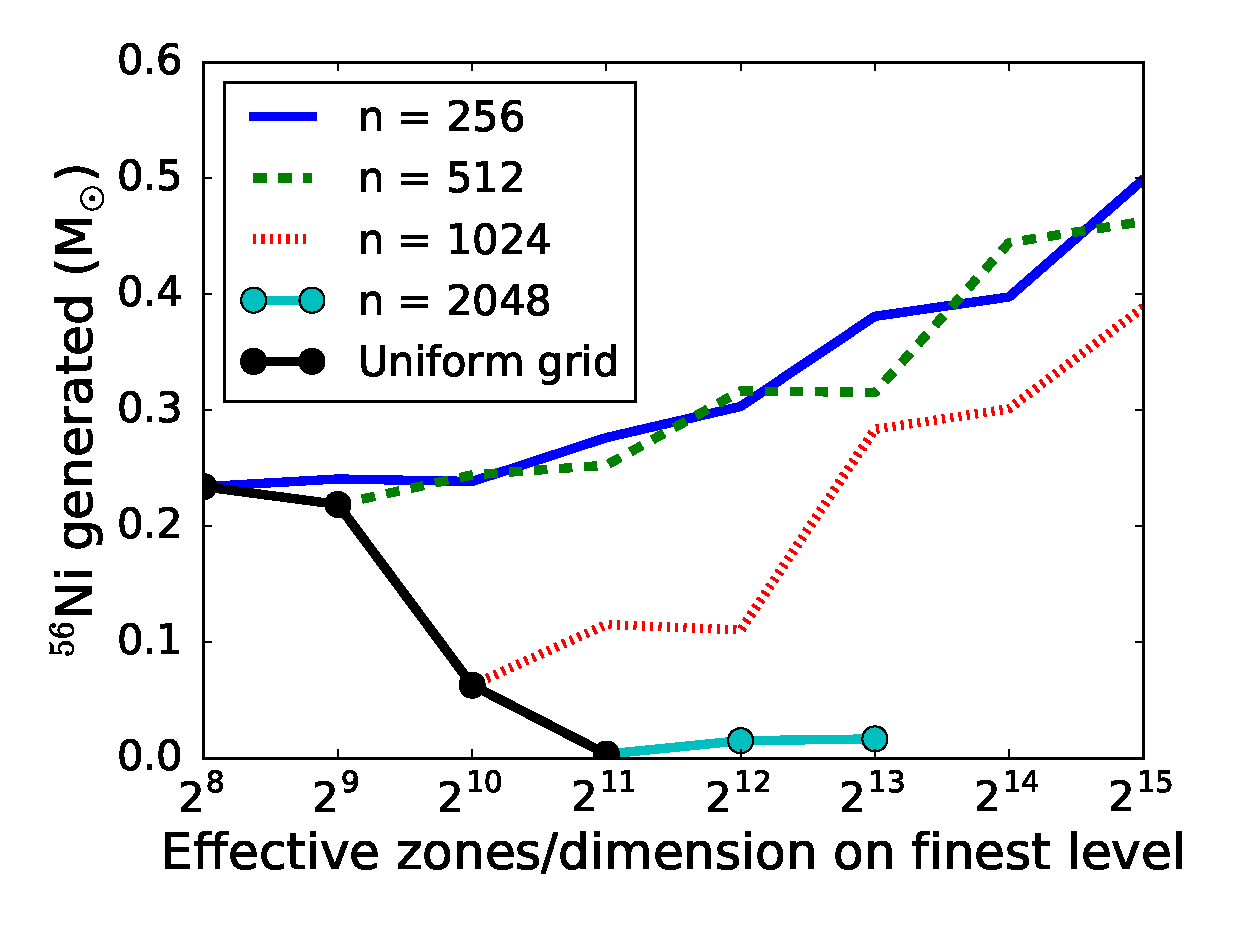
\includegraphics[scale=0.425]{{{plots/amr}}}
  \caption{Nickel production as a function of the simulation resolution. The solid
           black curve connects the points at uniform resolution. For each uniform
           resolution simulation, we include additional simulations using the adaptive
           mesh refinement criterion described in \autoref{sec:unstable_burning}.
           The horizontal axis is the effective number of zones per dimension on the
           finest level, which is the number of zones per dimension that would exist
           if the finest resolution was uniformly applied on the grid.
           \label{fig:amr}}
\end{figure}



%==========================================================================
% Conclusions
%==========================================================================
\section{Conclusions and Discussion}\label{Sec:Conclusions and Discussion}
\label{sec:conclusion}



\acknowledgments

This research was supported by NSF award AST-1211563 and DOE/Office of
Nuclear Physics grant DE-FG02-87ER40317 to Stony Brook. An award of
computer time was provided by the Innovative and Novel Computational
Impact on Theory and Experiment (INCITE) program.  This research used
resources of the Oak Ridge Leadership Computing Facility located in
the Oak Ridge National Laboratory, which is supported by the Office of
Science of the Department of Energy under Contract
DE-AC05-00OR22725. Project AST106 supported use of the ORNL/Titan
resource.  This research used resources of the National Energy
Research Scientific Computing Center, which is supported by the Office
of Science of the U.S. Department of Energy under Contract
No. DE-AC02-05CH11231. The authors would like to thank Stony Brook
Research Computing and Cyberinfrastructure, and the Institute for
Advanced Computational Science at Stony Brook University for access
to the high-performance LIred and SeaWulf computing systems, the latter
of which was made possible by a \$1.4M National Science Foundation grant (\#1531492).

This research has made use of NASA's Astrophysics Data System 
Bibliographic Services. In addition, this research has made use
of the AstroBetter blog and wiki.

\software{\amrex\ (\url{https://github.com/AMReX-Codes/Amrex}),
          \castro\ \citep{castro} (\url{https://github.com/AMReX-Astro/Castro}),
          \wdmerger\ \citep{wdmergerI} (\url{https://github.com/AMReX-Astro/wdmerger}),
          GCC (\url{https://gcc.gnu.org/}),
          python (\url{https://www.python.org/}),
          matplotlib \citep{matplotlib} (\url{http://matplotlib.org/}),
          yt \citep{yt} (\url{http://yt-project.org/})}

\facilities{OLCF, NERSC}

\clearpage

\bibliographystyle{../aasjournal}
\bibliography{../refs}

\end{document}
